% thesis.tex
%
% This file is root file for an example thesis written using the
% IIT Bombay LaTeX Style file.
% Created by Amey Karkare (21 June 2007)
%
% It is provided without warranty on an AS IS basis.

%=====================================================================
% Read: http://www.cse.iitb.ac.in/karkare/iitbthesis/
%    FAQ.txt     for frequently asked quetions
%    Changes.txt for changes
%    README      for more information
%=====================================================================

%=====================================================================
% DOCUMENT STYLE
%=====================================================================
% IITB PhD Thesis format default settings are:
%   12pt, one-sided printing on a4 size paper
\documentclass[openright,twoside]{iitkthesis}
% For two-sided printing, with Chapter starting on odd-numbered pages,
% use the following line instead:  
%%\documentclass[openright,twoside]{iitbthesis}

%=====================================================================
% OPTIONAL PACKAGES
%=====================================================================
% To include optional packages, use the \usepackage command.
% For e.g., The package epsfig is used to bring in the Encapsulated
%    PostScript figures into the document.
%    The package times is used to change the fonts to Times Roman;
%=====================================================================

%=====================================================================
%  Single counter for theorems and theorem-like environments:
%=====================================================================
\newtheorem{theorem}{Theorem}[chapter]
\newtheorem{assertion}[theorem]{Assertion}
\newtheorem{claim}[theorem]{Claim}
\newtheorem{conjecture}[theorem]{Conjecture}
\newtheorem{corollary}[theorem]{Corollary}
\newtheorem{definition}[theorem]{Definition}
\newtheorem{example}[theorem]{Example}
\newtheorem{figger}[theorem]{Figure}
\newtheorem{lemma}[theorem]{Lemma}
\newtheorem{prop}[theorem]{Proposition}
\newtheorem{remark}[theorem]{Remark}

\usepackage{minted}
\usemintedstyle{bw}

\usepackage{fontspec}
\setmonofont[Scale=0.85]{DejaVu Sans Mono}

\usepackage[sorting=none, maxbibnames=99, minbibnames=99]{biblatex}
\bibliography{citations}
\usepackage{amsmath}
\usepackage{lipsum}
\usepackage{float}
\usepackage[hidelinks]{hyperref}
\usepackage{microtype}
\usepackage[font=small,labelfont=bf]{caption}
\usepackage{fancyref}
\usepackage{color,soul} % for highlights
\usepackage{enumerate}
\usepackage{tabularx}

\setlength{\headheight}{15pt}

\expandafter\def\csname PY@tok@err\endcsname{}

\floatstyle{ruled}
\newfloat{program}{thp}{lop}
\floatname{program}{Figure}

\numberwithin{program}{chapter}

\BeforeBeginEnvironment{program}{\begin{singlespace}}
\AfterEndEnvironment{program}{\end{singlespace}}

%=====================================================================
% End of Preamble, start of document
%

\begin{document}

%=====================================================================
% Include the prelude for Title page, abstract, table of contents, etc
% You need to modify it to contain your details
% prelude.tex
%   - titlepage
%   - dedication (optional)
%   - approval sheet
%   - course certificate
%   - table of contents, list of tables and list of figures
%   - nomenclature
%   - abstract
%============================================================================


\clearpage\pagenumbering{roman}  % This makes the page numbers Roman (i, ii, etc)



% TITLE PAGE
%   - define \title{} \author{} \date{}
\title{Distributed Memory and CPU Management in Cloud Computing Environments}
\author{Shivanshu Agrawal}
\date{May, 2016}

%  - Roll number, required for title page, approval sheet, and
%    certificate of course work
\rollnum{11907688}

%   - The default degree is ``Doctor of Philosophy''
%     (unless the document style msthesis is specified
%      and then the default degree is ``Master of Science'')
%     Degree can be changed using the command \iitbdegree{}
\iitbdegree{Master of Technology}

%   - The default report type is preliminary report.
%      * for a PhD thesis, specify \thesis
\thesis
%      * for a M.Tech./M.Phil./M.Des./M.S. dissertation, specify \dissertation
%\dissertation
%      * for a DIIT/B.Tech./M.Sc.project report, specify \project
%\project
%      * for any other type, use  \reporttype{}
%\reporttype{ReportType}

%   - The default department is ``Unknown Department''
%     The department can be changed using the command \department{}
\department{Computer Science \& Engineering}

%    - Set the guide's name
\setguide{Prof. Mainak Chaudhuri}
\setguidedept{Department of Computer Science \& Engineering}

%   - once the above are defined, use \maketitle to generate the titlepage
\maketitle

%--------------------------------------------------------------------%
% CERTIFICATE
%     The first page after the title page.
\makecertificate

%--------------------------------------------------------------------%
% COPYRIGHT PAGE
%   - To include a copyright page use \copyrightpage
% \copyrightpage

%--------------------------------------------------------------------%
% ABSTRACT
\begin{abstract}
  To efficiently utilize the resources in a virtualized environment, they need to be overcommited. Overcommitment is the process of allocating more resources to a virtual machine, or a group of virtual machines than are physically present on the host. It is based on the premise that most of the Virtual Machines will use only a small percentage of the resources allocated to them at a given time. However, situations may arise when the resources required by the virtual machines are more than the physical resources present on the machine. The performance of the Virtual Machines will be severely impacted in these situations. Most cloud providers generally have Service Level Agreements (SLAs) with their clients and hence cannot allow virtual machines to deliver a poor quality of service.

In this thesis, we explore the problem of overcommitment of the CPU and memory resources. We propose a distributed resource scheduler (DRS) which uses techniques such as memory ballooning and virtual machine live nigration to solve the problems in CPU and memory overcommitment. We design an architecture for DRS which is horizontally scalable and describe the techniques involved in monitoring and memory ballooning aspects of the DRS.

\end{abstract}

%--------------------------------------------------------------------%
% DEDICATION
%   Dedications, if any.
\begin{dedication}
Dedicated to\\
my parents
\end{dedication}

% Acknowledgements
\begin{acknowledgments}
I would like to extend my sincere gratitude towards my thesis supervisors, Prof. Mainak Chaudhuri and Prof. Sumit Ganguly for their guidance, constant support and encouragement. This thesis would not have been possible without them.

I thank the Department of Computer Science and Engineering, IIT Kanpur for providing the necessary infrastructure and congenial environment facilitating this research work.

I also thank Tejas Gandhi for providing invaluable help in setting up Openstack, Adarsh Jagannath for various useful discussions we had which proved instrumental in the progress of this thesis, Abhimanyu Arora  for working on a part of this thesis together with me, and all my fellow batchmates for the delightful time we spent together and making my stay at IITK memorable.

I am forever indebted to my family for everything in my life.

\hfill \hfill \textbf{Shivanshu Agrawal}
\end{acknowledgments}

%--------------------------------------------------------------------%
% CONTENTS, TABLES, FIGURES
\tableofcontents
\listoftables

\cleardoublepage
\phantomsection \label{listoffig}
\addcontentsline{toc}{chapter}{List of Figures}
%\listof{program}{List of Figures}
\listoffigures

\cleardoublepage\pagenumbering{arabic} % Make the page numbers Arabic (1, 2, etc)


%=====================================================================
% Include the technical part of the report
%% \include{chap_intro}             % Chapter 1: Introduction
%% \include{chap_others}            % Other chapters as required
%% \include{chap_conclusions}       % Finally the summary & conclusions

%=====================================================================
% APPENDIX
%  Appendices, if any, must precede the cited literatures.
%  Appendices shall be numbered in Roman Capitals (e.g. Appendix IV)

%% \appendix
%% \include{appendix_something}          

%=====================================================================
% PUBLICATIONS
%  publications if any may be listed after the literature cited.
%% \include{mypubs}

%=====================================================================
% ACKNOWLEDGMENTS
%   This is the last item in the thesis. It should be signed by
%   author, with date.


\chapter{Introduction: Virtualization and Resource Management in Cloud}
\label{chap:intro}

With the advent of large scale cloud computing, the users can get compute resources on demand with flexible pricing models. Cloud vendors pool their massive hardware resources and provide virtual machines on top of it to the users. To best utilize the resources of a virtualized cloud infrastructure, resource overcommitment is used. Allocating more virtual resources to a machine or a group of machines than are physically present is called resource overcommitment.

Since most applications will not use all of the resources allocated to them at all the times, most of the resources of a cloud provider will remain idle without overcommitment. Hence, this approach is more profitable and less wasteful. Orthogonal to overcommitment is the fact that cloud vendors have to satisfy some SLAs (Service Level Agreements) which they have with the users i.e.\ the promised resources should be available to the users whenever they need it. Distributed resource scheduling (DRS) is used to meet these SLAs.

Apart from the public cloud offerings like Amazon Web Services and Microsoft Azure, many companies and educational institutions are virtualizing their IT infrastructure to create private clouds. Private clouds may have less strict SLA's but require resource scheduling to enhance performance of the virtual machines. Overcommitment without resource management may lead to degradation in performance.

\section{Virtualization}
Virtualization is one of the driving technologies behind IaaS (Infrastructure as a Service). Virtualization makes it possible to run multiple operating systems with different configurations on a physical machine at the same time. 

To run virtual machines on a system, a software layer called hypervisor or virtual machine monitor (VMM) is required. The hypervisor has the control of all the hardware resources and can take away resources from one VM to give it to another. The hypervisor also maintains the state of all the VMs at all the times. It does these by trapping all the privileged instructions executed by the guest VM and emulating the resource they access. The hypervisor is responsible for emulating all the hardware devices and providing proper resource isolation between multiple machines running on the same physical machine. 

There are three different techniques used for virtualization \cite{horne2007understanding} which mainly differ in the way they trap the privileged instructions executed by the guest kernel.

\begin{enumerate}
\item \textbf{Full Virtualization with Binary Translation.} In this approach, user mode code runs directly on CPU without any translation, but the non-virtualizable instructions \cite{Popek:1974:FRV:361011.361073} in the guest kernel code are translated on the fly to code which has the intended effect on the virtual hardware.

\item \textbf{Hardware Assisted Full Virtualization.}To make virtualization simpler, hardware vendors have developed new features in the hardware to support virtualization. Intel VT-x and AMD-V are two technologies developed by Intel and AMD respectively which provide special instructions in their ISA (Instruction Set Architecture) for virtual machines and a new ring privilege level for VM. Privileged and sensitive calls are set to automatically trap to the VMM, removing the need for either binary translation or paravirtualization. It also has modified MMU with support for multi level page tables \cite{bhargava2008accelerating} and tagged TLBs. 

%TODO: cite xen
\item \textbf{Paravirtualization.} This technique requires modification of the guest kernel. The non-virtualizable/privileged instructions in the source code of the guest kernel are replaced with hypercalls which directly call the hypervisor \cite{barham2003xen}. The hypervisor provides hypercall interfaces for kernel operations like memory management, interrupt handling, and communication to devices. It differs from full virtualization, where unmodified guest kernel is used and the guest OS does not know that it is running in a virtualized environment.  
\end{enumerate}


Hypervisors can be bare-metal hypervisors or hosted hypervisors. A Bare-metal
hypervisor runs directly on the physical hardware while the hosted hypervisor runs
on top of conventional operating systems. There are several hypervisors available
in the market with VMWare ESX and Xen \cite{barham2003xen} being the popular bare-metal hypervisors,
while KVM-QEMU \cite{kivity2007kvm, bellard2005qemu} being a popular hosted hypervisor which runs on top of the Linux
operating system. KVM is a kernel module providing support for hardware assited virtualization in Linux while, QEMU is a userspace emulator. KVM uses QEMU mainly for emulating the hardware \cite{Habib:2008:VK:1344209.1344217}. So, both these pieces of software work together as a complete hypervisor for linux. KVM-QEMU and Xen are open source while ESX is proprietary. For the
purpose of this thesis, we will refer to KVM-QEMU wherever hypervisor is used unless specified otherwise.

Virtualization provides a number of benefits other than resource isolation, 
which makes it the fundamental technology behind IaaS.
\begin{enumerate}
\item It provides the ability to treat disks of virtual machine as files which can be easily snapshotted for backup and restore.
\item It provides ease of creation of new machines and deployment of applications through pre-built images of the filesystem of the machine.
\item Virtual machines can be easily migrated or relocated if the physical machines may require maintenance or develop some failure.
\item Ease in increasing the resource capacity (RAM or CPU cores) of the machine at runtime by CPU or memory hotplug \cite{Hansen_hotplugmemory}, or otherwise.
\item Since the hardware resources are emulated by the hypervisor, there is an opportunity for overcommitment of CPU and memory resources here. 
\end{enumerate}

\subsection{Memory Overcommitment and Ballooning} \label{ballooning}

In memory overcommitment, more memory is allocated to the virtual machines(VM) than is
physically present in hardware. This is possible because hypervisors allocate
memory to the virtual machines on demand. KVM-QEMU treats all the running VMs as
% TODO: give the line number reference for malloc in qemu source
processes of the host system and uses malloc to allocate memory for a VM's
RAM. Linux uses demand paging for its processes, so a VM on bootup will allocate
only the amount of memory required by it for booting up, and not its whole capacity. 

On demand memory allocation in itself is not enough to make memory overcommitment a
viable option. There is no way for the hypervisor to free a memory page that has been freed by the guest OS. Hence a page once allocated to a VM always remains
allocated. The hypervisor should be able to reclaim free memory from the guest machines, otherwise the memory consumption of
guest machines will always keep on increasing till they use up all their memory
capacity. If the memory is overcommited, all the guests trying to use their maximum
capacity will lead to swapping and very poor performance.

There exists a mechanism called \textit{memory ballooning} to reclaim free memory from guest machines. This is possible through a device driver that exists in guest operating system and a backend virtual device in the hypervisor which talks to that device driver. The balloon driver takes a target memory from the balloon device. If the target memory is less than the current memory of the VM, it allocates $(current-target)$ pages from the machine and gives them back to the hypervisor. This process is called balloon inflation. If the target memory is more than the current memory, the balloon driver frees required pages from the balloon. This process is called balloon deflation. Memory ballooning is an opportunistic reclamation technique and does not guarantee reclamation. The hypervisor has limited control over the success of reclamation and the amount of memory reclaimed, as it depends on the balloon driver which is loaded inside the guest operating system.

The Memory ballooning technique leverages modified guest kernel as it uses an extra device driver and hence falls under Paravirtualization. But the virtio balloon driver \cite{russell2008virtio} exists in the linux source code since version 2.6 and a backend balloon device exists in QEMU to facilitate ballooning. The virtio drivers can be installed additionally in a Windows system.


\subsection{CPU Overcommitment}
CPU overcommitment happens through time sharing of CPU cores on a physical machine by multiple VMs. The virtual CPU cores for a VM are called vCPU. Most hypervisors allow multiple virtual machines to share same physical CPU core for multiple vCPUs.
QEMU-KVM runs one vCPU thread per guest CPU \cite{qemu-multi}. The thread scheduling onto physical CPU is handled by the host operating system. Time sharing CPU cores can incur a performance penalty, which is measured by the time a vCPU spends in the ready queue, i.e.\, the time for which a vCPU is ready to be scheduled but does not get scheduled. This time is called the \textit{steal time} as it represents the CPU cycles that have been stolen from the vCPU. If the guests on a host experience high steal, the CPU of the host is overloaded.

\section{Virtual Machine Live Migration}
VM live migration \cite{Clark:2005:LMV:1251203.1251223} is a technique to migrate a running VM from one host to another without shutting it down. Live migration involves migrating the disk, memory and CPU states of the running VM to the destination host and resuming the VM there. Migrating disk can be as easy as just copying the disk to destination or using a file-system shared over the network like Network File System (NFS). There are two popular techniques for migrating the VM memory and state:

\begin{enumerate}
\item \textbf{Pre-Copy Live Migration.} It follows an iterative page copying technique wherein first, all the pages of the VM are copied to the destination. From next iteration onward, only the pages which were dirtied during the previous iteration are copied to the destination. This process continues till the page dirtying speed is less than the page transfer speed. Then the VM at the source is stopped, remaining dirty pages and VM state is copied to the destination, and the VM is resumed at the destination. QEMU-KVM uses pre-copy live migration \cite{qemu-migration}.

\item \textbf{Post-Copy Live Migration.} The VM is stopped at the source, its state is copied to the destination, and the VM resumed there. The pages of the VM are transferred to the destination in background, with the pages that are immediately demanded by the VM via page fault given the highest priority in transfer. Thus, the performance of the VM is degraded before its working set is transferred.
\end{enumerate}

The migration time of a VM is the time taken to resume the VM on the destination after triggering the migration. There is also a small amount of downtime involved in live migration in which the VM is neither running on the host, nor on the destination. Live migration of VMs connected to a network is especially tricky because the new VM has to assigned the same IP address and all the packets have to rerouted to the new destination without any delay to prevent packet loss and downtime of any service running inside the VM which uses the network.
\Fref{tab:live-migration} lists some other key differences between the two techniques \cite{yabusame}.

\begin{table}[hbt]
\caption{Differences between pre-copy and post-copy live migration}
\label{tab:live-migration}
\begin{center}
\begin{tabularx}{0.91\textwidth}{XX}
\hline\noalign{\smallskip}
Pre-Copy & Post-Copy \\
\noalign{\smallskip}
\hline
\noalign{\smallskip}
Total migration time = (RAM size/link speed) + overhead + non-deterministic  (depending on dirtying pattern) & Total migration Time = (RAM
size/link speed) + overhead \\ \\

Worst downtime =  (VM state time) + (RAM size/link speed) & Worst downtime = VM state time \\ \\

It can cope with network or system failure. & In case of network or system failure, VM cannot be recovered. \\
\hline
\end{tabularx}
\end{center}
\end{table}


\section{Resource Management in Cloud}

Resource management is an essential technique to utilize the underlying hardware of the cloud efficiently. The role of the resource manager is to manage the allocation of physical resources to the virtual machines deployed on a cluster of nodes in a cloud. Different resource management systems may have different aims depending upon the needs. For a private cloud like in an educational institution, the most common aim might be to maximize performance of the virtual machines while minimizing the operational costs of the cloud infrastructure. 

Minimizing operational costs involves minimizing the number of physical machines used. This can be achieved through overcommitment of resources. Resource overcommitment comes with some new problems like hotspot elimination and where to schedule new incoming VMs to minimize chances of hotspot. If the total capacity of the virtual machines running on a physical machine is more than the total capacity of the physical machines, a situation may arise wherein the VMs may want to use a sum total of more resources than are present. Not satisfying those resource requirements may lead to violation of SLAs and poor performance of the VMs. This situation is called a hotspot. A distributed resource scheduler (DRS) is a piece of software that runs on different nodes in the cluster and handles dynamic resource allocation to different VMs in the cluster.

Memory ballooning and live migration of VM can help in mitigating hotspots. The basic idea is that if a VM is short on memory, ballooning can be used to take away some memory from another guest on the same host which has some free memory and give it to the needy guest. If none of the guests have any free memory, the host is overloaded. A guest has to be migrated from this host to another host while taking into account the overall load of the cluster. This might sound simple, but there are several challenges involved in this process. Some of the challenges are determining the amount of free memory a VM can give away without affecting its own performance, determining whether benefits of migration are more than performance loss, selecting which virtual machine to migrate such that maximum benefit is achieved out of the migration, selecting destination host to minimize the chances of future migrations, filtering intermittent spikes from resource usage graph of VMs to determine their actual load profile and distributed monitoring of VMs which can scale to a large number of machines. In this thesis, we address large scale monitoring and ballooning of virtual machines. 

\section{Organization of this Thesis }
The rest of the thesis is organized as follows. Chapter 2 describes related work that has been done in this area. Chapter 3 consolidates the requirements of a DRS, outlines our approach to building the DRS, and proposes a decentralized and scalable architecture for it. Chapter 4 describes the details of implementation of the monitoring and autoballooning components of our DRS. Chapter 5 analyses the monitoring and autoballooning components of the DRS through experimental data. Finally, Chapter 6 concludes the work done in this thesis and provides some insights on possible extensions to this work.

\subsection*{Summary}
In this chapter, we discussed the different technologies behind cloud computing and looked at how they are used. We have looked at how resource overcommitment helps in utilizing the hardware efficiently and why resource management is essential for overcommitment to work. We have also identified several problems and challenges related to resource management which have been resolved in this thesis.
\chapter{Related Work}
\label{chap:related}

\section{Auto-Ballooning in Xen}
Xen is a popular open-source, bare-metal hypervisor which was developed by University of Cambridge Computer Laboratory in 2003 and was the first hypervisor to support paravirtualization. Support for full vritualization was later added to it. Xen has autoballooning feature which works via the autoballoon driver that exists in the Linux kernel. Autoballooning implementation in our work has some key differences to autoballooning in Xen, which have been discussed later. It is important to understand both techniques for comparison. To understand Xen hypervisor's method of autoballooning, it is first essential to understand transcendent memory in Linux.

\subsection{Transcendent Memory (tmem)}
Transcendent memory (tmem) \cite{magenheimer2009transcendent} is a type of memory which the linux kernel cannot directly enumerate, track or directly address, but helps in more efficient utilization of memory by a single kernel or load-balancing of memory between multiple kernels in a virtualized environment. 

The implementation of tmem is divided into two parts - frontend and backend. Frontend provides the interfaces for different types of data which can be stored provided by tmem to the kernel, while backend is the underlying implementation of storage/retrieval methods. Two basic operations provided by the frontend are 'put' and 'get'. If the kernel wants to save some data into tmem, it uses the 'put' operation while 'get' is used to retrieve the data.

\subsubsection{Tmem Frontends}
There are two tmem frontends in the Linux kernel which cover two major types of kernel memory - \textit{anonymous pages} and \textit{file backed pages}.
\begin{enumerate}
\item \textbf{Cleancache:} Cleancache is used for storing pages which are backed by files on a disk. A kernel can choose to reclaim such pages at the times of memory pressure. These pages are evicted from memory. If the same page is to be used again, a page fault happens and it is fetched from the disk. Before evicting such a page, the kernel can choose to store it in cleancache. If the operation succeeds, the page can possibly be reclaimed from tmem at any later time, otherwise it has to be reclaimed from disk, if needed

Cleancache data in tmem is ephemeral i.e.\ tmem can choose to discard any cleancache data at any point of time. Later, when a kernel wants its data back from tmem, if tmem has already discarded that data, the kernel can fetch it from the disk.

\item \textbf{Frontswap:} Frontswap is used for storing swap pages. Linux swap subsystem stores anonymous pages in a swap device when it needs to evict them. Whenever the swap subsystem of the Linux kernel wants to swap a page to swap device, it can send the page to tmem instead. If the operation succeeds, the page is written to tmem, otherwise it goes to the swap device. Frontswap provides a guarantee that a page stored in it can be reclaimed at any later point of time, and it will not be discarded.
\end{enumerate}

\subsubsection{Tmem Backends}
There are multiple backends for tmem - \textit{zcache}, \textit{transcendent memory for Xen}, and \textit{RAMster}. Tmem was originally developed for Xen with Xen backend. The other backends were created later. For autoballooning, we are only concerned with the Xen backend.

Tmem backend for Xen works in a virtualized environemnt under the Xen hypervisor to share the spare hypervisor memory amongst the running VMs. In a virtualized environment, the memory is allocated to the running VMs on demand. Some memory is also reserved for the hypervisor to run. Thus, it may have some free memory which is not used by anyone nd can be used for Tmem. This will result in faster swap out/in and page reclamation for the guests under memory pressure. This plays an important part in autoballooning of VMs and differentiates autoballooning in KVM from Xen, as we will see in the later sections.

\subsubsection{Frontswap Self Shrinking}

When kernel swaps out a page, it assumes that the page will go to disk and may remain there for long time even if it is not used again as kernel assumes disk space is less costly and abundant. But if the page has gone to frontswap, it is taking up valuable memory which might be better used elsewhere. To resolve this problem, \textit{frontswap-self-shrinking} is used. When a guest kernel is under normal memory pressure, it uses partial swapoff interface to bring the pages which were swapped to tmem back to guest's memory. This frees tmem for use by other guests which might be under memory pressure.

\subsection{Auto-Balloon Mechanism}
Autoballooning in Xen requires transcendent memory. In each guest, a autoballoon driver is present. A thread of the driver runs periodically in some fixed (configurable) time interval which sets the target size of the guest.


$$Target = Committed\ pages + Reserved\ pages + Balloon\ reserved\ pages$$


\textit{Committed pages} are the pages which are used by some process and may reside either in memory or swap. \textit{Reserved pages} are the pages reserved from normal usage by the kernel. \textit{Balloon reserved pages} form the memory reserved by the balloon driver to provide some extra memory for the kernel caches and some room to grow for any process that may demand more memory in the future. It defaults to 10\% of the total memory size of the guest. If the target is less than the current RAM, the guest is ballooned down, else it is ballooned up. There is a hysteresis counter which represents the number of iterations it will take for the machine to balloon down to target. So, each time self-ballooning process runs, 
$$Memory = Current - \frac{Current-Target}{hysteresis\ counter}$$

Hysteresis counter is different for ballooning up and down. There is also a\textit{min usable MB} parameter, below which machines cannot be ballooned.

It is important to note here that Xen autoballooning is proactive in nature. Even if none of the guests is under memory pressure, it reclaims free/idle memory from the guests. This may seem wasteful as the memory reclaimed when there is no memory pressure on the host may have been better used by the original guest for page caches. But this is compensated by the fact that the reclaimed memory, if not given to any other host, will go to tmem, which will lead to faster swap in/out for all the guests. So, the reclaimed memory is shared by all the guests and can be used by them depending on the need. This kind of ballooning is not possible for KVM because there is no tmem backend for QEMU-KVM. Thus, QEMU-KVM requires reactive ballooning.

\section{Memory Management in VMware ESX}
VMware was founded in 1999 when it launched its proprietary hypervisor which used binary translation techniques for x86 virtualization. They later released an enterprise class bare metal hypervisor called VMware ESXi. ESX has very robust memory management and it introduced several novel techniques as early as 2003 which are still being used and have been implemented in other platforms. The techniques used by ESX to manage memory \cite{waldspurger2002memory} of its guests and facilitate memory overcommitment have been very briefly described here.

\subsection{Memory Reclamation Techniques}
ESX uses several memory reclamation techniques.
\begin{enumerate}
\item \textbf{Content-Based Page Sharing:} In a virtualized environment, several guests might be running common OS and some common applications which means that there would be lots of pages having the same content. Instead of keeping separate copies of these pages for separate guests, the duplicate pages are deleted and only one copy of the page is kept which is marked Copy-On-Write(COW). When any of the guests attempts to write to that page, a new copy of the page is created by the kernel which is then modified.

Linux kernel has KSM(Kernel Same-Page Merging) \cite{ksm} which performs the same task and is used in virtualization by QEMU-KVM.
\item \textbf{Memory Ballooning:} Memory Ballooning has been explained in Section \ref{ballooning}
\item \textbf{Page compression:} In this case, the content of the page is compressed and stored. When the page is accessed, its content is decompressed.
\item \textbf{Demand Paging:} ESX server has a swap daemon which handles hypervisor level swapping. The swap daemon gets the target swap levels of each VM from the swapping policy and selects the pages that need to be swapped. 

\end{enumerate}

\subsection{Memory Reclamation Policies}
The ESX server defines four memory states depending upon which it employs the memory reclamation techniques.

\begin{enumerate}
\item \textbf{High:} More than 6\% of the total memory of the hypervisor is free at this point. Only page sharing is employed in this state.
\item \textbf{Soft:} Free memory is between 6\% and 4\%. Page sharing is active. Balloon driver also starts reclaiming idle memory.
\item \textbf{Hard:} Free memory is between 4\% and 2\%. The hypervisor now aggressively starts reclaiming memory through swapping. Page compression also becomes active. So, on page reclamation, if it is compressible or shareable, it is compressed/shared otherwise it is swapped out.
\item \textbf{Low:} Below 1\% free memory. Along with memory reclamation, ESX also blocks any new memory allocation by any guest.
\end{enumerate}

One important point of contention here is which pages and how many pages to reclaim from each guest. For determining how much memory to reclaim from each guest, ESX uses a share based allocation technique. After getting the amount of memory to reclaim, it chooses the pages to reclaim randomly.

\subsubsection{Share-Based Allocation}
Under share-based allocation, each guest is allocated some number of shares for memory. A machine is guaranteed a minimum resource fraction equal to its fraction of the total shares in the system. So, in case of memory pressure, memory should be revoked from the guest which has the fewest shares per allocated page. This may lead to idle clients having large number of shares hoarding memory unproductively while active clients having fewer shares suffer under memory pressure. 

To resolve this situation, ESX imposes a tax on idle memory of guests. Thus, for a client with $S$ shares and $P$ allocated pages  out of which a fraction $f$ are active, the shares-per-page ratio $R$ is
$$R = \frac{S}{P(f+k(1-f))}$$
where the idle page cost is $k=1/(1-\tau)$ and tax rate $\tau$ is between 0 and 1. Tax rate controls the maximum fraction of idle pages that can be reclaimed from a VM. The default value of $\tau$ is $0.75$.
\subsubsection{Idle Memory Calculation} \label{working-set}
For calculating share per page ratio effectively, idle memory calculation for each guest is required. ESX uses statistical sampling to estimate the working set size of each VM. At the start of the sampling period, a small number $n$ of a VM's pages are selected randomly using uniform distribution. Accesses to these pages are tracked by the hypervisor by incrementing a counter $t$ on every page access. At the end of the sampling period, the fraction of working set is estimated as $f=t/n$.

\section{VMware Distributed Resource Management}
VMware created DRS \cite{gulati2012vmware} for their hypervisor which is responsible for allocation of the physical resources to a set of virtual machines deployed in a cluster of hosts. The key capabilities of their DRS are a hierarchical resource pool abstraction, automatic initial placement of VM, and dynamic load balancing of VMs based on their fluctuating demands. Some of our work is inspired by VMware's DRS and aimed at fixing some of its limitations. Hence, this section provides an appropriate background for the next chapter.

\subsection{Resource Model}
Each VM in VMware DRS has three resource control parameters. \textit{Reservation} specifies a minimum guaranteed amount of a particular resource which will always be available to the VM. \textit{Limit} specifies the maximum amount of a resource that can be allocated to a VM. \textit{Shares} specify the relative importance of the VMs similar to the shares in memory allocation of ESX described in the previous section.

The resources in a cluster are divided into resource pools which are used for dividing the aggregate capacity of the cluster into a group of VMs. The resource pool forms a  hierarchical tree structure with leaves as the actual VMS. The resource pool can represent the hierarchical structure of the oraganization.

\subsection{DRS Algorithm}
The DRS algorithm runs every five minutes. It first divides the resources of the cluster amongst the resource pool in a process called \textit{divvying}. It computes the reservation, limit, and shares of each pool. To distribute the resources, it is important to calculate the demand of each VM, which can be used to calculate the total load on the cluster. The working set of a VM is used as it's memory demand. The working set is calculated in the way explained in Section \ref{working-set}. The CPU demand of a VM is computed as its actual CPU consumption plus a scaled portion of the  time it was ready to execute, but it spent in the ready queue due to contention.

$$ CPU_{demand} = CPU_{used} + \frac{CPU_{run}}{CPU_{run}+CPU_{sleep}}*CPU_{ready}$$

The divvying algorithm works by dividing the resource at the parent resource pool amongst the children. It executes in two phases. In the initial phase, it aggregates demand values of the VMs from leaves up to the root. At each step, the demand values are updated to be not less than the reservation and not more than the limit. The second phase proceeds in a top-down manner and resources (limit and reservation) of parents at each level are divided such that they are in proportion to shares of the siblings. 

After divvying, the DRS load-balances the cluster based on a metric called dynamic entitlement. Dynamic entitlement is equal to the demand of the VMs if demands of each VM in the cluster can be met, otherwise it is a scaled down value of a VM’s demand based on its shares. It is computed by running the divvying algorithm at the resource pool tree using the cluster capacity as the resource. Then, normalized entitlement is calculated for each host. For a host $h$, normalized entitlement $N_h$
 is defined as the sum of per VM entitlement of all VMs running on $h$ divided by the host capacity.
 $$N_h = \Sigma \frac{E_i}{C_h}$$
 $N_h$ values are per-resource. $N_h < 1$ signifies that the host has some unused capacity for that resource, while $N_h > 1$ means that it is overloaded for that resource. The DRS then calculates the cluster wide imbalance $I_c$ as the weighted sum of the standard deviation of all $N_h$ values for CPU and memory resources. If memory is highly contested, it's weight is more. If CPU is highly contested, CPU's weight is more. If none are highly contested, both have equal weights. The higher weighted resource gets a weight of $three$ while the lower weighted resource gets a weight of $one$. These values were decided by experimentation.

The DRS then tries to minimize the cluster wide imbalance $I_c$ by considering all possible VM migrations (trying out all possible guest VM , destination host pairs). The best VM migration is selected, applied to cluster’s state, and another move is selected. This process continues till no beneficial moves remain, or enough moves have been selected for this pass, or the cluster imbalance $I_c$ is below a threshold. Additionally, DRS also does a cost-benefit analysis of each move where it filters out the moves with higher migration cost than benefit in terms of decreasing load imbalance.

\subsection{Limitations of VMware DRS}
The major limitation of VMware DRS is scaling, which is due to several reasons. There is a central controller for the cluster which monitors all the hosts and virtual machines. In a cloud scale, where the hosts can grow to thousands in number and VMs to tens of thousand, a central machine monitoring all of the components and taking all the decisions is not possible. Apart from this, in making a decision, the DRS considers all possible VM migrations. The time for running this algorithm grows exponentially with the number of VMs and hence cannot scale. On top of all this, the controller is a single point of failure for the whole cluster in this design.

Another limitation of VMware DRS is that it manages only CPU and memory resources. Other resources like network bandwidth, and disk I/O, which can affect the performance of a VM,can also be considered.

\section{Other Works}
%TODO: citations here
Sandpiper \cite{wood2009sandpiper} is a system for automating the task of detecting hotspots and migrating VMs in response to hotspots. For VM migration, Sandpiper takes three resources into consideration - CPU, memory and network bandwidth. The empty volume of each host is calculated as $empty\_vol = (1-cpu)(1-net)(1-mem)$. It calculates $volume$ occupied by a VM as $$vol = \frac{1}{1-cpu} * \frac{1}{1-net} * \frac{1}{1-mem}$$. It then calculates volume to size ratio (VSR) of each VM, where size is a VMs memory footprint. The VM with the maximum VSR from the host having the least $empty\_vol$ is migrated to the host having the maximum $empty\_vol$. Some of the problems and anomalies in this approach have been explored \cite{mishra2011theory}.

CloudScale \cite{shen2011cloudscale} uses long-term resource demand prediction models to predict the resource demands of virtual machines in future based on the previous resource usage data. It handle conflicts by proactive migration of virtual machines based on the predicted demands. Tan et al. \cite{tan2011exploiting} propose a similar approach where they use a Principal Component Analysis (PCA) based approach to predict the long-term resource usage profiles of the VMs using the measurements obtained from a commercial data center. They formulate the VM placement problem as a bin-packing problem and propose to place VMs using variance reduction. But in doing so, they assume that the resource usages of the VMs remains constant, which may not be the case in reality.

Vector Dot \cite{singh2008server} is a load balancing algorithm for handling multi-dimensional resource constraints in a virtualized infrastructure. It expresses the normalized resource requirements of machines as multi-dimensional vectors. It then uses the dot product of the resource usage vector (RUV) of the host and the resource requirement vector (RRV) of the guest to choose an appropriate host-VM mapping. To ensure balanced usage of resources, the RRV of the guest should be complementary to the RUV of the host. The anomalies with this approach have been discussed and improvements have been proposed \cite{mishra2011theory}. But these studies do not take scaling into consideration and are not distributed enough to handle the cloud scale. They also do not consider the performance degradation that happens during live migration.

\subsection*{Summary}
In this chapter, we have discussed the autoballooning mechanism implemented in the Xen hypervisor and how it is different from the autoballooning in KVM. We have discussed the techniques which VMware ESX implemens for memory management and distributed resource scheduling. We have also explored some other important works in this area and their drawbacks.
\chapter{Architecture and Design of DRS}
\label{chap:design}

\section{Functions of DRS}
Distributed resource scheduler is responsible for handling the dynamic resource allocation requirements of VMs on the cloud. The job of a DRS can be divided into three categories:

\begin{enumerate}
\item \textbf{Monitoring.} Monitoring is essential for detecting the resource requirements of individual guest machines running on the cloud and detecting hotspots on physical hosts which make up the cluster. It has to be fine-grained enough to detect changes in the load profile of the hosts and guests. It has to be coarse enough to filter short-terms changes in the resource requirements of the guests. It will also regularly update the load statistics of the host in a shared data store which can be used to get a global account of the cluster state at any point of time which will be useful in making decisions about live-migration.
\item \textbf{Memory Management.} For all the guests running on the same host, DRS will manage their ever changing memory demands. Autoballooning is an essential technique for the DRS to perform this aspect of its functionality. This part of DRS will look at the memory usage statistics of all the guests, figure out which VMs need more memory and which VMs have idle memory, and try to meet the demands of each VM by inflating/deflating its balloon.
\item \textbf{Hotspot Mitigation.} In the case of a hotspot, this part of DRS is responsible for selecting an appropriate guest to migrate and the best destination for it based on the resource usage data of all the machines present in the cluster.
\end{enumerate}

\section{Goals and Non-Goals}
\textit{Goal:} Develop a DRS for private clouds which makes the best use of the resources available i.e. provides the resources to the machines on a best effort basis according to the priority/importance of each VM. If the cluster is not fully loaded, the demands of all the VMs can be satisfied but if the load is more than the capacity, the VMs will have to do with less resources than promised. In case of an overload, all the VMs with the same priority across the cluster should be treated equally in resource allocation. 

\textit{Goal:} The DRS design should be decentralized so that it is easily able to scale up to a cluster having thousands of physical hosts and there is no single point of failure in the system.

\textit{Non-goal:} Minimizing the number of machines used. Though using less machines will save power because the unused machines can be turned off, the goals of power management are orthogonal to the goals of our DRS and can be treated separately.

\textit{Non-goal:} For the purpose of this thesis, we have considered balancing only memory and CPU resources. Other resources like disk I/O, and network bandwidth have not been taken into account.

\section{Architecture Overview}
%TODO: insert a figure here.
The DRS architecture described below is fully decentralized, which is a key requirement for scaling it up to thousands of hosts. Decentralization also prevents any single point of failures. Each host in the cluster makes its own decision about the guest machines on that host and the other hosts co-operate with it to make that decision successful.
The DRS is divided into three components based on the three types of job mentioned earlier that it has to perform. 

\begin{figure}[!ht]
  \centering
  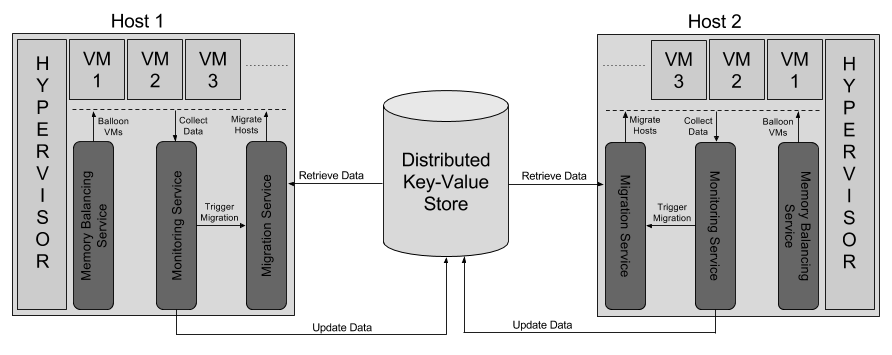
\includegraphics[width=\textwidth]{arch.png}
  \caption{Architecture of the DRS}\label{fig:mem}
\end{figure}

\subsection{The Monitoring Service}
A \textit{monitoring service} runs on all the hosts of the cluster. On each host, it collects the resource usage statistics of all the VMs on the host and the total resource usage of the host. It also filters out the short-term changes in the resource usage and figures out the changes in the load profile. It also detects any hotspot and triggers the migration service to perform its task of migrating a guest away from the host. The service also accommodates (start monitoring) any new guest that is migrated to a host. 

The service talks to a distributed key-value store to regularly update the resource usage statistics of the host it is running on. The key-value store should be updated only when there is a significant change in the resource usage profiles of the host, which could affect the decision making of live migration. Small changes in the resource usage are unnecessary to track as they will not affect the decision making. Short-term spikes in the resource usage can adversely affect the live-migration decisions by misrepresenting the resource usage.

\subsection{The Memory Balancing Service}
A \textit{memory balancing Service} runs on all the hosts. On each host, the service looks at the memory usage statistics of all the VMs running on the host provided by the monitoring service. It figures out which hosts require more memory and which hosts have some idle memory. It then balances the memory by inflating/deflating the balloons of the VMs.

If the demands of all the VMs can be satisfied, balancing takes idle memory and gives it to the needy. If the demands of all the VMs cannot be satisfied i.e. there is a hotspot on the host, the service calculates the entitled memory based on the priority of each VM running on the host for each guest. Entitled memory may be less than the memory needs of a guest. Then the service distributes memory according to the entitlement. 

The service also tries to make space by freeing memory for any new guest that is to be migrated to the host. Notably, this service does not do anything to resolve hotspots. It just tries to balance memory amongst the guests present on the host. Hotspot mitigation is left to the migration service. If there is a hotspot, some guest(s) may get migrated out of the host, leaving free memory for other VMs.

The memory management requires a separate service while CPU management does not. There are two reasons for this.
\begin{enumerate}
\item vCPU of each VM is handled as a thread by the hypervisor and hence scheduled according to its process scheduling policy, while there is no such system for memory.
\item Memory, once consumed by a VM, is not reclaimed automatically by the hypervisor, while this is not the case with the CPU resources. Each vCPU thread gets a time slice to run which is decided by the hypervisor and the CPU is taken away from the thread after the time slice ends.

\end{enumerate}

\subsection{The Migration Service}
This service runs on all the hosts and is triggered by the \textit{monitoring service} when there is a hotspot on the host. It collects the resource usage statistics of all the other hosts in the cluster from the data-store to which the monitoring services of all the hosts write. This data would be just a few key-value pairs per host and hence, very small. Using this data (and some other), it tries to find out the best migration (guest VM-destination host pair) performing which will improve some metric representing the resource requirement satisfaction or the overall performance of the VMs on the cluster. The service talks to the memory balancing service on the destination host to free required memory for the incoming guest, and then it migrates the guest to the destination. The migration service requires resource usage details of the entire cluster to make an informed decision on migration.

\subsection*{Summary}
In this chapter, we have discussed the functions and goals of a DRS. We have also proposed a decentralized architecture for DRS which can scale well and is free of single point failures.
\chapter{Implementation of Monitoring and Auto-Ballooning}
\label{chap:impl}

For the purpose of this thesis, we describe the implementation and experimentally evaluate only the monitoring and autoballooning parts of the DRS. The following sections describe the implementation details of these two components.

\section{Monitoring}
As we discussed in Chapter \ref{chap:design}, the monitoring component runs on each host and monitors the host and the guests running on that host to detect hotspots. The next few sections discuss which metrics are monitored, why they are monitored, and how they are monitored. Our implementation is done in the \textit{Python programming language}. The monitoring service runs periodically in every fixed time interval which is configurable. The default interval is set to then seconds. We will refer to this time interval as the \textit{monitor interval} in the rest of this document.

\subsection{Host Monitoring}
Monitoring the host is simple because the Linux kernel exposes much of the needed information stored in its internal data structure through procfs \cite{procfs}. Procfs is a filesystem in the Linux kernel, and hence can be accessed using the standard filesystem syscalls or through higher level API's that exist in almost all programming languages for this purpose. Since the DRS is running on the host, it has unhindered access to all the information in procfs.

\subsubsection{CPU Monitoring} \label{sec:cpumon}
For monitoring the CPU usage, we use the information in the  \textit{/proc/stat} file. The \textit{/proc/stat} file has the following fields capturing how much time CPU spent doing what task \cite{procfs}.

\begin{itemize}
\item \textbf{user:} time spent in executing normal processes in the user mode
\item \textbf{nice:} time spent in executing processes with positive nice value in the user mode
\item \textbf{system:} time spent in executing processes in kernel mode
\item \textbf{idle:} time for which the cpu was idle
\item \textbf{iowait:} time spent in waiting for I/O to complete
\item \textbf{irq:} time spent in servicing interrupts
\item \textbf{softirq:} time spent in servicing software interrupts
\item \textbf{steal:} time spent waiting involuntarily. This metric is relevant when the kernel running under virtualization, and its vCPU thread has to wait in the ready queue because the host CPU is overloaded.
\item \textbf{guest:} time spent running a normal guest (VM)
\item \textbf{guest\_nice:} time spent running a guest (VM) with positive nice value.
\end{itemize}
The time is measured in kernel jiffies. Jiffy is a counter that ticks on every timer interrupt. The interrupt frequency is 100Hz in majority of the systems.
From the above values, we can get the total time that has passed, and time for which the cpu was busy.
\begin{multline*}
 Total Time = user + nice + system + idle + iowait \\ + irq + iowait + irq + softirq + steal + guest + guest\_nice
\end{multline*}
$$ Busy Time = user + nice + system + irq + softirq + guest + guest\_nice$$

The $Total Time$ calculated here is the total time since the start of the system. Hence this will give the average cpu usage since the start of the system, which is not a useful metric for us. The average cpu usage in the previous monitor interval is more useful. To calculate that, we keep the $Total Time$ and $Busy Time$ at the previous monitor interval and subtract those values from the current values. So, 
$$
PrecentageCpuUsage = \frac{Busy Time - Previous Busy Time}{Total Time - Previous Total Time}*100$$

\subsubsection{Memory Monitoring} \label{impl:hostmemmon}
Memory usage information is present in the \textit{/proc/meminfo} file \cite{procfs}. For monitoring, we need several memory metrics which are described below.
\begin{itemize}
\item \textbf{Total memory:} The total usable memory present on the host. Present in the first line of the \textit{/proc/meminfo}.
\item \textbf{Used memory:} Total memory used by the host. This includes the memory used by the VMs, host's own processes and the page caches. This can be calculated by subtracting free memory, which is present in the second line of \textit{/proc/meminfo} file, from total memory.
\item \textbf{Available memory:} This provides an estimate of how much memory is available to any new application that will be started on the system. This is different from free memory because used memory also contains page caches, which can be reclaimed in case no free memory is left and an application requires more memory. Some of the slab memory used by the kernel is also reclaimable. The estimate also accounts for the fact that the system needs some page cache to function well, and that not all reclaimable slab can be reclaimed. It is present in the third line of \textit{/proc/meminfo} file.

Available memory is an important metric for us, because it basically tells us how much memory is available for the new VMs. It is better than free memory, because free memory does not take into account page caches which can be reclaimed.

\item \textbf{Hypervisor Load:} This is an important metric because we want to have a lower bound on how much memory is available for the hypervisor to function. We call this memory \textit{hypervisor reserved memory}. While calculating the amount of memory that is free for VMs to use, we do not want to use the memory that is reserved for the hypervisor.

For calculating the hypervisor load, we first calculate the VM load i.e.\ the amount of memory used by the virtual machines on the system. The VM load is calculated by looking at the RSS (resident set size) of all the virtual machines running on the host. Since QEMU-KVM treats each VM as a separate process, we need to get the RSS of all the processes which are running a virtual machine. The \textit{/proc/[pid]/statm} file has this information for each process. After calculating the VMlLoad, the hypervisor load is calculated as
$$Hypervisor Load = max(Hypervisor Reserved, Used Memory - Page Caches - VMLoad)$$

\item \textbf{Load Memory: } This metric represents the total memory that is loaded and hence, not available for use by any new VM or for existing VMs. It is calculated as
$$ 
Hypervisor Extra = max(Hypervisor Reserved-Hypervisor Load, 0)$$
$$Load Memory = (Total Memory - Available Memory - Idle Memory) + Hypervisor Extra$$

\item \textbf{Idle Memory: } Idle Memory is the memory which has been consumed by the VMs but is sitting idle inside the VM and can be ballooned out. Thus, it can be used by the existing VMs or any new VM that is migrated to the host. Its calculation is described later in the Section \ref{sec:guestmon}.
\end{itemize}

\subsection{Guest Monitoring} \label{sec:guestmon}
Monitoring a VM is more complex than monitoring the host because some of the metrics needed are not exposed by the VM to the host in any conventional way. Host operating system just gets to see the process abstraction of each virtual machine. So, the host has only as much information about each guest as it has about the rest of the processes running on it. In the next two sections, along with which metrics have been monitored, we have discuss some new techniques which we use to get some of the information from the guest VMs.

\subsubsection{CPU Monitoring}
CPU monitoring for a guest VM is straightforward because the host OS has the scheduling information for each process it is running. This information is exposed by the procfs. The metrics related to CPU utilization measured are discussed below.
\begin{itemize}
\item \textbf{Busy Time:} This is the time for which any of the vCPUs of the VM was scheduled onto any of the physical CPUs of the host. The scheduling information for each thread of a process is present inside the \textit{/proc/[pid]/task/[tid]/schedstat} file \cite{procfs}. We can get the busy time for each thread in nanoseconds from here. Adding the busy time for all the vCPU threads gives us the total busy time. The total time elasped has already been calculated in Section \ref{sec:cpumon}. We do calculation similar to Section \ref{sec:cpumon} to get the busy time percentage in previous monitor interval for all the guests.
\item \textbf{Steal Time:} Steal time \cite{ehrhardt2013cpu} is the time for which a vCPU thread waits in the ready queue while the CPU is busy executing some other process. Steal time has direct correlation to the amount of load on CPU and is useful in predicting whether the CPU is overloaded. Steal times for each thread is present inside the \textit{/proc/[pid]/task/[tid]/schedstat} \cite{procfs}. For each VM, we add the steal times of all its vCPU threads and calculate the average steal time percentage in the previous monitor interval.
\item \textbf{Estimated CPU Demand:} Estimated CPU demand is useful for predicting the amount of CPU a VM can consume if the host is not overloaded i.e.\ the steal time is 0. This value will be helpful during migration to check whether the CPU demands of the VM can be satisfied by the destination. It is calculated by adding a scaled value of steal percentage to the current busy percentage.
$$Estimated CPU DemandPrecent = \frac{Busy Time}{Total Time}*(1+\frac{Steal Time}{Total Time})*100 $$
\end{itemize}
\subsubsection{Memory Monitoring}
Getting the memory usage statistics is difficult because the host has no information about the memory management of the guest. The host only knows the amount of memory allocated by each guest. For calculating the idle memory of each guest, we need the amount of \textit{available memory} inside the VM.

One way for a guest VM to expose some information to the host is through a device driver. In a virtualized environment, all the devices available to a VM are virtual devices which are emulated by the hypervisor. So, a device driver running inside the VM can send some information to the device which is emulated by the hypervisor. The virtio balloon driver in the Linux kernel has a way of exposing the memory statistics to the host. It gives the total memory, free memory, swap in, major page faults, minor page fault metrics. We have modified the balloon driver to expose the available memory metric to the host too. We have also modified the backend virtio balloon hardware in QEMU to take the Available Memory metric from the balloon driver inside the guest. 
The following metrics related to the memory usage of the VMs are monitored. Figure \ref{fig:mem1} shows the relative sizes of different memory metrics calculated.
\begin{figure}[h]
  \centering
  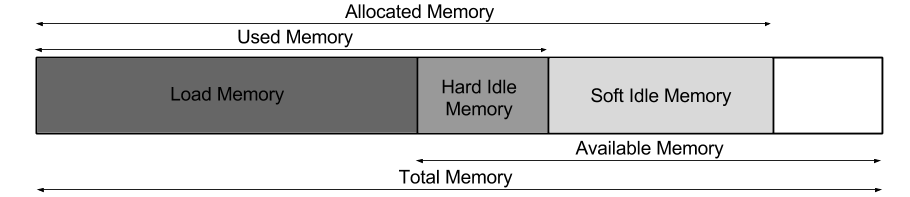
\includegraphics[width=\textwidth]{mem1.png}
  %\includegraphics{right-graph}
  \caption{Relative sizes of different types of memory metrics}\label{fig:mem1}
\end{figure}
\begin{itemize}
\item \textbf{Maximum Memory:} This is the maximum memory that the guest can have. The guest cannot be ballooned up after this point. We obtain this metric by using the API QEMU provides for this purpose.
\item \textbf{Current Memory:} This the amount of memory the guest has after taking the ballooned memory into account. From the point of view of the guest, this is its total memory, which can be increased or decreased by ballooning. The maximum limit for the current memory is the maximum memory. The \textit{total memory} statistic obtained through the virtio balloon driver represents this metric.
\item \textbf{Used Memory:} This is the memory which is being used by the guest. It includes all the page caches along with the memory being used by the processes inside the guest.
\item \textbf{Available Memory:} This is the amount of available memory inside the guest. The concept of available memory has been discussed in Section \ref{impl:hostmemmon}. We have modified the virtio balloon driver to obtain this metric.
\item \textbf{Allocated Memory:} This is the amount of memory of the guest that is backed by physical memory on the host. Allocated memory is different from current memory because the memory is allocated to the vritual machines on demand. This also may not equal to the used memory of the guest. Without ballooning, the memory, once allocated to a guest, is not reclaimed from it. So, the usage of a guest may keep on changing, but the allocated memory will always be equal to the maximum used memory in the guest's lifetime. Allocated memory is helpful in calculating the idle memory.

The allocated memory is calculated by looking at the virtual memory maps of the QEMU-KVM process corresponding to each VM. This information is present inside the \textit{/proc/[pid]/smaps} file \cite{procfs} for each process. The RAM of the guest VM is allocated by the QEMU process by doing a malloc of the size of maximum memory. Thus, it is one big contiguous chunk of memory in the heap memory of the process. From the information about different memory sections of the process present in this file, we look for the heap memory chunk of the size of VM's maximum memory. The RSS (resident set size) of this chunk of memory gives us the amount of memory in the VM that is backed by physical storage. 

In this chunk of allocated memory, there is some amount of memory that QEMU uses to store some metadata about the pages of the guest VM. Hence, this entire memory is not available to the guest. This part of memory cannot be reclaimed by ballooning. This overhead is constant and depends on the maximum memory size of the guest. We call this overhead as QEMU overhead. QEMU overhead needs to be deducted from the RSS. We use a piecewise continuous function to model the QEMU overhead. The values for the QEMU overhead in different scenarios were determined experimentally.
\[
QEMU Overhead =
  \begin{cases} 
      \hfill 200 MB    \hfill & \text{if $maxmem <= 4GB$} \\
      \hfill 300 MB \hfill & \text{if $ 4GB < maxmem <= 10GB$} \\
      \hfill 400MB \hfill & \text{if $ 10GB < maxmem <= 18GB$} \\
      \hfill 500MB \hfill & \text{if $ maxmem > 18GB$} \\
  \end{cases}
\]
$$ Allocated Memory = RSS - QEMU Overhead$$
\item \textbf{Load Memory:} This is the amount of memory that is loaded i.e.\ is being used by the processes of the guest and hence the current memory should not go below this point. 
$$Load Memory = Current Memory - Available Memory$$
\item \textbf{Idle Memory:} Idle memory is the amount of memory that is allocated, but is not being used by the guest, and hence, can be reclaimed. A lower bound on the current memory of the guest has been kept to avoid ballooning so much memory out of it that it is unable to function. This bound is called \textit{guest reserved}. So,
$$LowerBound = max(LoadMemory, GuestReserved)$$
$$Idle Memory = max(Allocated Memory - LowerBound, 0)$$
Based on how the idle memory is reclaimed, it can be divided into two types - hard idle memory and soft idle memory. Their importance and the difference between them have been explained in Section \ref{sec:bal}.
\end{itemize}

\subsection{Hotspot Detection and Key-Value Store Updation}
The hotspot detection algorithm should be robust enough not to generate false alarms. A simple threshold based algorithm which takes absolute or average values into account can raise many false alarms. Andreolini et al. \cite{andreolini2009dynamic} have shown the drawbacks of such algorithms and proposed a more robust statistical model to detect changes in the load profile of a machine which is based on the CUSUM (Cumulative Sum) algorithm \cite{page1957estimating}. We have used this algorithm for detecting hotspots and the time to update the key-value store. The algorithm is described below for the sake of completeness.

The hotspots due to memory overload are detected using the load memory metric of the host. The values for load memory are recorded in ever monitor interval to form a time series. Exponential average of the data is calculated as
$$ \mu_i = \alpha * loadmem_i + (1-\alpha)\mu_{i-1}$$
The value of $\alpha$ has been chosen to be $0.1$. The algorithm detects abrupt increase in  $\mu_i$ using $d_i$.
$$d_0 = 0;\ d_i = d_{i-1}+(loadmem_i - (\mu_i+K))$$
$d_i$ measures all the deviations from $\mu_i$ that are greater than $K$. $K=\frac{\Delta}{2}$ where $\Delta$ is the minimum shift to
be detected. It has been set to ($0.005*TotalMemory$) to detect minimum 1\% change in the value of $loadmem$. Change in the load profile of the host is triggered when $d_i > H$ where $H = h\sigma$, $h$ being a design parameter and $\sigma$ being the standard deviation of the time series upto that point. We have set $h=7$, which means that the load profile change is detected in an average of 14 samples \cite{andreolini2009dynamic}.
When the load-profile changes, the key-value store is updated with $totalmem - loadmem$. When the load profile changes and $(\mu_i > 0.8 * totalmem)$, hotspot is triggered and the migration service becomes active.

The hotspots in the CPU usage are also calculated in a similar way. The only difference is that the CUSUM algorithm runs on the steal time of all the guests, and any guest can trigger hotspot when its load profile changes and its $Average Steal Time > 10\%$. Additionally, the CUSUM algorithm runs on the busy time of the host to trigger the updation of the key-value store. The value stored in the key-value store is $(Number Of CPUs*100-BusyTimePercentage)$

\section{Auto-Ballooning}
Ballooning is a technique for increasing or decreasing the current memory of a guest. Auto-Ballooning is the process of automatically balancing memory amongst multiple guests running on a system by taking some memory from the idle guests and giving it to the needy guests. Auto-Ballooning is the most essential component for memory overcommitment.

\subsection{Hard Ballooning and Soft Ballooning} \label{sec:bal}
Depending upon the type of memory reclaimed ballooning can be classified into two types - hard ballooning and soft ballooning. Soft ballooning is the process of reclaiming memory which is free inside the guest while hard ballooning is the process of reclaiming memory which is used inside the guest.

\begin{align*}
&SoftLowerBound = max(Used Memory, Guest Reserved)\\
&Soft Idle Memory = max(Allocated Memory - SoftLowerBound, 0)\\
&Hard Lower Bound = max(Load Memory, Guest Reserved)\\
&Hard Idle Memory = max(Used Memory - Hard Lower Bound, 0)
\end{align*}

For soft ballooning, the guest is ballooned down to $(Current Memory - Soft Idle Memory)$, which will reclaim the SoftIdleMemory. To reclaim HardIdleMemory, the guest has to be ballooned down to $(Used Memory - Hard Idle Memory)$. Thus, ballooning down a guest from current memory to $(Current Memory - Soft Idle Memory)$ will reclaim SoftIdleMemory. After this, ballooning down from  $(Current Memory - Soft Idle Memory)$ to $Used Memory$ will reclaim no memory. Then, ballooning down from used memory to $(Used Memory - Hard Idle Memory)$ will reclaim the HardIdleMemory. Figure \ref{fig:mem2} shows the two different types of ballooning.

\begin{figure}[hb]
  \centering
  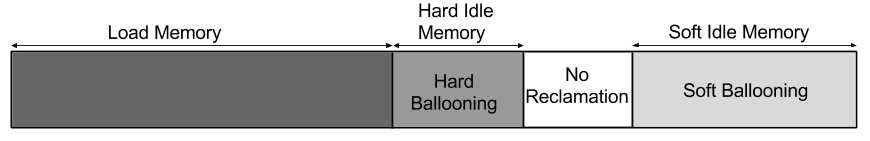
\includegraphics[width=\textwidth]{mem2.png}
  %\includegraphics{right-graph}
  \caption{Soft and hard ballooning}\label{fig:mem2}
\end{figure}

\subsection{Auto-Ballooning Algorithm}
The autoballooning algorithm first identifies the guests with idle memory and the guests which need more memory. We have already described the method of calculating the idle memory earlier. We identify needy guests as the ones whose average load memory is greater than a certain threshold. We have kept the threshold to $90\%$ of the current memory of the guest. Needy guests are ballooned up in intervals of $10\%$ of their current memory. Total needed memory is the sum total of the memory needed by all the needy guests(which is 10\% of the current memory for each needy guest).
\[
isNeedy(guest) =
  \begin{cases}
  	  \hfill True \hfill &  \text{$LoadMemory \ge 0.9*CurrentMemory$}\\
      \hfill False \hfill & \text{otherwise} \\
  \end{cases}
\]
$$ NeededMemory = 0.1*CurrentMemory$$

The \textit{host unused memory} is the amount of memory on the host which is neither used by/allocated to any guest nor is being used by the host, and hence, can be given away to any host by ballooning it up. Ballooning up a guest reduces the host unused memory, while ballooning a guest down decreases it. It is calculated as follows.
\begin{align*} 
Host Unused Memory = Available &Memory - Hypervisor Extra\\
&or\\
Host Unused Memory = Total Memory& - Load Memory - Total Idle Memory
\end{align*}
Auto-Ballooning can be triggered in two cases -  $(Host Unused Memory < 0.1*Total Memory)$ or $(Total Needed Memory>0)$.  The first case is important to keep the amount of swapped memory on the host low. To handle the first case, first the soft idle memory and then the hard idle memory form the guests is ballooned out till the $(Host Unused Memory < 0.2*Total Memory)$. If the idle memory is exhausted before this 20\% memory becomes unused, swapping is inevitable and the job of resolving it is left to the migration service.

%TODO: A figure here explaining ballooning algo in all the cases.
In the second case, either there is a needy guest or memory needs to be reclaimed for a guest which would be migrated to the machine. Both the situations are similar except that when memory is reclaimed for an incoming guest, there is no needy guest to be ballooned up. Depending on the needed memory and idle memory, three situations can arise.
\begin{enumerate}
\item $\mathbf{Total Needed Memory \le Total SoftIdleMemory.}$ The requirements of each needy guest can be satisfied by just soft-ballooning. So, the idle guests are ballooned down to reclaim the needed memory and then, the needy guests are ballooned up.
\item $\mathbf{TotalSoftIdleMemory < Total Needed Memory \le Total HardIdleMemory.}$ First, all the soft idle memory is ballooned out. Then, the rest of the needed memory is divided among the guests with hard idle memory in proportion of their hard idle memory. So, memory reclaimed by hard ballooning for a guest is given by
$$ NeedAfterSoftBallooning = TotalNeededMemory - TotalSoftIdleMemory$$
$$ Hard Reclaim = \frac{GuestHardIdleMem*NeedAfterSoftBallooning}{TotalHardIdleMemory}$$
Here, $GuestHardIdleMem$ is the hard idle memory for that particular guest, while $TotalHardIdleMem$ is the total hard idle memory. The reason hard ballooning is treated differently from soft ballooning is because soft ballooning is not supposed to have any affect on the performance of the guest as it takes away only the free pages. On the other hand, hard ballooning also reclaims some of the page caches, which might have some effect on the performance of the guest.
\item $\mathbf{Total Needed Memory > TotalHardIdleMemory.}$ This case implies that there is a hotspot on the host. Since the demands of all the guests cannot be satisfied, the memory is given to them or reclaimed from them based on their entitlement. The \textit{entitled memory} of each guest is calculated as
$$ EntitledMemory = GuestMaximumMemory*MemoryOvercommitmentRatio$$
After this, the idle memory and needed memory calculation is done again. 
$$ Idle Memory = max(Current Memory - Entitled Memory, 0)$$
\[
Needed Memory =
  \begin{cases}
  	  0 \ \ \ \ \ \ \ \ \ \ \ \ \   \text{if $!isNeedy(guest)$}\\
      0 \ \ \ \ \ \ \ \ \ \ \ \ \  Current Memory > Entitled Memory\\
      min(0.1*CurrentMemory,\\ \ \ CurrentMemory - Entitled Memory) \ \ \  \text{otherwise} \\
  \end{cases}
\]
Then, the idle memory is ballooned out of the guests and the needed memory is provided to the needy guests.

\subsection*{Summary}
In this chapter, we looked at the different techniques we use to monitor various metrics for hosts and guests. These metrics are used to trigger hotspot and make the ballooning service active. We also looked at the CUSUM based algorithm used to filter out unecessary spikes in the resource usage profiles of the host. In the end, we also discussed our technique of autoballooning.
\end{enumerate}


\chapter{Experimental Evaluation}
\label{chap:experiment}
We have built our DRS for the QEMU-KVM hypervisor. It uses the \textit{libvirt} APIs for managing the virtual machines and \textit{Openstack} \cite{openstack} mainly for cloud management and software defined networking along with live-migration support. For the distributed key-value store, we use \textit{etcd} \cite{etcd}. We have conducted several experiments to determine the effectiveness of our DRS. The experiments relating to monitoring and auto-ballooning aspect of the DRS have been described below.

\section{Experimental Setup}
Our experimental setup consists of six physical machines. Each physical machine has an 8 core Intel Core i7 3.5GHz CPU, 16 GB memory, 1Gbps NIC and runs the 64 bit Ubuntu 14.04 with Linux kernel version 3.19 . We have installed Openstack on these 6 nodes such that one of the nodes is the controller node(runs the Openstack management services) and the other five are the compute nodes (run the actual VMs). The nodes are connected to a gigabit local network, which they use for transferring data while live migration and for communicating with the outside network. The disks of all the VMs reside on a shared NFS server, and hence, live migration needs to just transfer the memory of the VM between the hosts, and not the disks. Each of the compute nodes also run the DRS software created by us. The controller and two separate nodes (separate from the controller and the compute nodes) run etcd, with a cluster size of three, which provides a fault tolerance of degree one \cite{etcd-ad}. All the VMs that we use run 64 bit Ubuntu 12.04 cloud image. The VMs can be of two sizes - 1 vCPU with 2 GB RAM(small) or 2 vCPU with 4 GB RAM(large).

There are three types of workloads run by these VMs. One workload is memory intensive, one is CPU intensive and one of the workloads is a mix of the two. The memory intensive workload is a program written by us which consumes a total of 1800MB. The program runs in two phases - the allocation phase and the retention phase. The allocation phase starts when the program starts. In the allocation phase, the program tries to allocate 100MB memory using \textit{malloc} and then sleeps for two seconds. This step is performed iteratively till the allocated memory has reached 1800MB. Notably, it may take more than 18 iterations for the allocation to reach 1800MB because malloc will return \textit{null} if it cannot allocate memory due to shortage of memory and the program will sleep for two more seconds. So, the length of the allocation phase depends on the availability of memory. After the allocation phase, retention phase starts, where the program retains the allocated memory for 300 seconds, and does no more allocations. After the retention phase, the program ends. We will refer to this workload as \textit{usemem}.

For the other two types of workloads, we have chosen two SPEC CPU 2006 V1.2 benchmarks \cite{Henning:2006:SCB:1186736.1186737}. For CPU intensive workload, we run the \textit{libquantum} benchmark. The libquantum benchmark tries to solve certain computationally hard problems using the simulation of a quantum computer. At runtime, the benchmark consumes 100\% of a vCPU and about 50MB memory. For the CPU and memory intensive workload, we use the \textit{mcf} benchmark. The mcf benchmark solves the single-depot vehicle scheduling problem in the planning process of public transportation companies using the network simplex algorithm accelerated with a column generation. At runtime, the mcf benchmark consumes 100\% of a vCPU and about 1800MB memory.

Large VMs run two workloads in two separate threads simultaneously, while the small VMs runs only one workload in a single thread. Each thread randomly chooses a workload from the three workloads described above, runs it and calculates the time it took to run the workload, sleeps for a randomly chosen time between 0 and 90 seconds, and then repeats this process. Each compute node has four large VMs and three small VMs. Keeping aside one core and two GB memory for the hypervisor, this gives us an overcommitment ratio of $1.57$ for  both CPU and memory.

\section{Results}
The experiment that we ran was to determine the effectiveness of autoballooning in memory overcommitment. For this, we monitored two hosts named compute2 and compute3 respectively, running seven VMs as described in the previous section. We disabled live-migration in the DRS on the both hosts. On compute3, autoballoning was also disabled. We compare the results obtained after running the experiment for about 17 hours.

\subsection{Analyzing Auto-Ballooning}
Figure \ref{fig:mem} shows the different memory metrics of compute2 and compute3 hosts plotted against time. From these graphs, the most remarkable difference that we can see is in the swap memory on both the machines. On compute3, the swap memory rose to very high levels of about 7GB, which is equal to the amount of memory we have overcommited. On compute 2, the swap memory remained very low throughout the experiment, remaining below 1GB most of the time and never going above 1.5GB. On compute3, the total used memory remains almost constant and equal to maximum memory, while it keeps on fluctuating on compute2. This is because memory, once allocated, cannot be reclaimed on compute3.
\begin{sidewaysfigure}[!htbp]
  \centering
  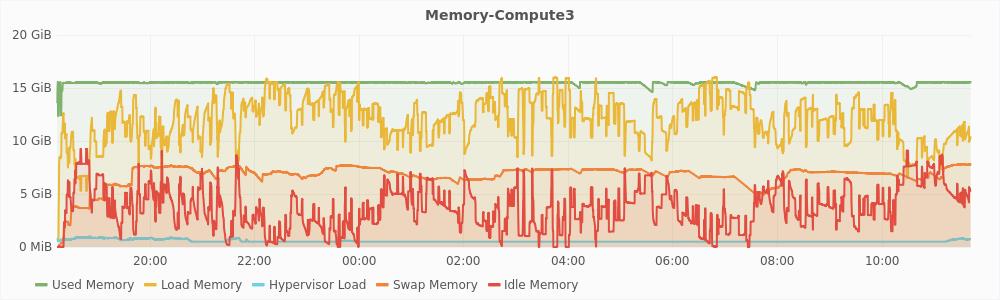
\includegraphics[width=\textwidth]{mem-compute3.png}
   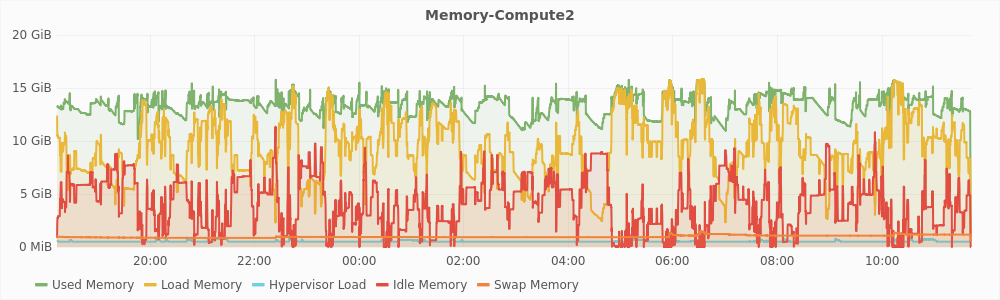
\includegraphics[width=\textwidth]{mem-compute2.png}
  \caption{Graphs showing different memory metrics of compute3 (autoballooning disabled) and compute 2 (autoballooning enabled). X-axis represents the time at which the value was recorded, Y-axis shows the value.}\label{fig:mem}
\end{sidewaysfigure}

Figure \ref{fig:cpu} shows the CPU usage of compute2 and compute3 plotted against time. In the graph, a few hours after starting the experiment, the CPU usage of compute3 is consistently low, while compute2 makes better use of the CPU. This is because of high levels of swap on compute 3. The mcf and usemem workloads spend more time in performing I/O and hence are not able to utilize the CPU efficiently.

\begin{sidewaysfigure}[!htbp]
  \centering
  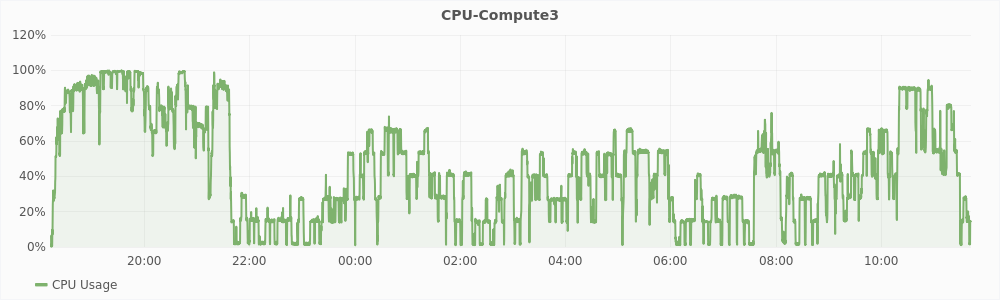
\includegraphics[width=\textwidth]{cpu-compute3.png}
  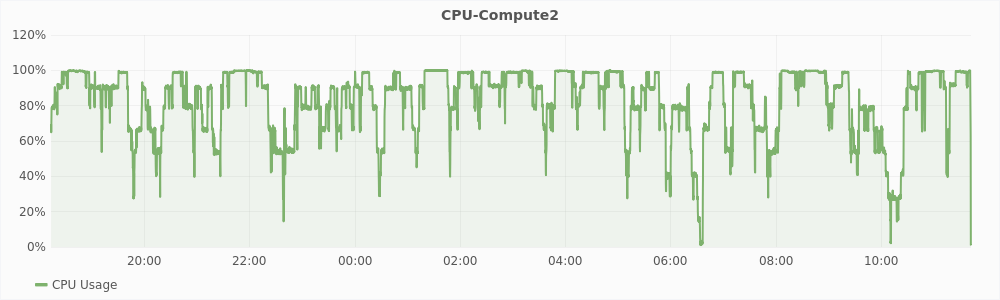
\includegraphics[width=\textwidth]{cpu-compute2.png}
  \caption{Graphs showing cpu usage of compute3 (autoballooning disabled) and compute2 (autoballooning enabled). X-axis represents the time at which the value was recorded, Y-axis shows the value.}\label{fig:cpu}
\end{sidewaysfigure}
Table \ref{tab:count} lists the number of time each workload ran on both the machines. Libquantum and mcf are CPU intensive. On compute2, CPU intensive workloads ran 303 times compared to 287 times on compute3 in the same time interval. Mcf and usemem are memory intensive. On compute2, memory intensive workloads ran 357 times compared to 289 times on compute 3 in the same time interval. It clearly shows that there was better utilization of the CPU and memory resources on compute2 resulting in a better overall throughput. 

\begin{table}[hbt]
\caption{Number of times each workload ran during the experiment}
\label{tab:count}
\begin{center}
\begin{tabularx}{0.91\textwidth}{XXX}
\hline\noalign{\smallskip}
Workload & Count-compute3 & Count-compute2\\
\noalign{\smallskip}
\hline
\noalign{\smallskip}
libquantum & 153 & 198\\

mcf & 134 & 105 \\

usemem & 155 & 252 \\
\hline
\end{tabularx}
\end{center}
\end{table}


\begin{sidewaysfigure}[!htbp]
  \centering
  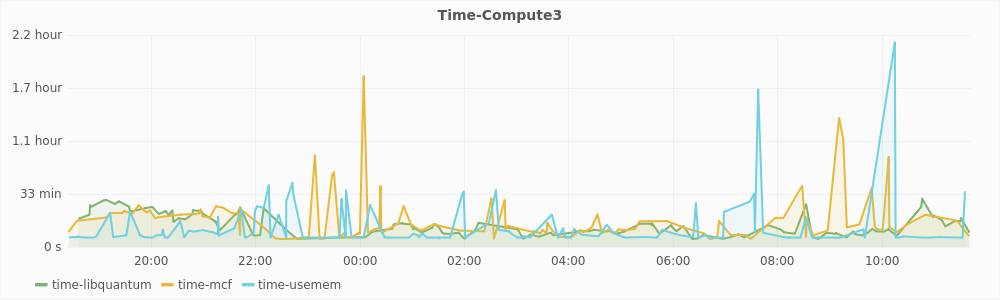
\includegraphics[width=\textwidth]{time-compute3.png}
  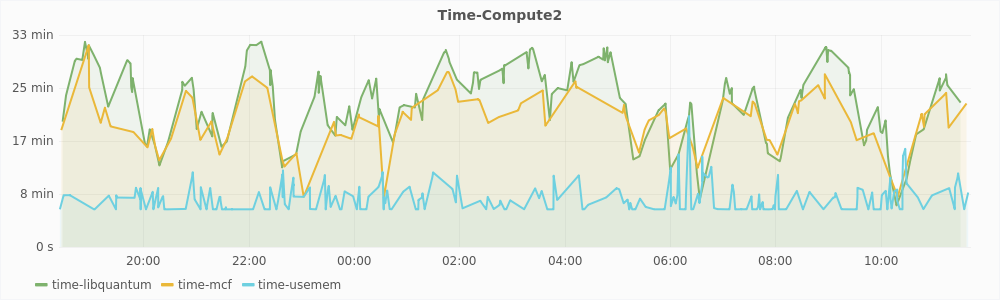
\includegraphics[width=\textwidth]{time-compute2.png}
  \caption{Graphs showing the time taken by different workloads on the two hosts. The values greater than two hours have been filtered out from the compute3 graph for the sake of visibility. X-axis represents the time at which the value was recorded, Y-axis shows the value.}\label{fig:time}
\end{sidewaysfigure}


\begin{table}[!htbp]
\caption{Mean time taken by each workload to run}
\label{tab:mean}
\begin{center}
\begin{tabularx}{0.91\textwidth}{XXX}
\hline\noalign{\smallskip}
Workload & Mean-compute3 & Mean-compute2\\
\noalign{\smallskip}
\hline
\noalign{\smallskip}
libquantum & 14.5 min & 23.7 min\\

mcf & 39.6 min & 20.3 min\\

usemem & 12.8 min & 7.9 min \\
\hline
\end{tabularx}
\end{center}
\end{table}

The graphs in Figure \ref{fig:time} show the time it took for the workloads to run plotted against the time at which the workload completed. In the graph for compute3, we can see that the time to complete the memory intensive workloads - mcf and usemem can grow to more than two hours while it always remains below 33 minutes on compute2. On top of this, some of the very large values have been filtered out from the graph of compute3. There were three such values for the mcf benchmark, which were greater than 9 hours. On the contrary, the libquantum workload performs better on compute3. This is because libquantum does not require much memory and the CPU on compute3 is relatively free because the other workloads do not utilize it well.
Table \ref{tab:mean} shows the mean time it took for the workloads to run. As expected, the libquantum performs better on compute3 while the other workloads perform better on compute2. But mean time is not a good metric to compare the effectiveness of autoballooning. Throughput is a better metric.

\subsection{Analyzing CPU Hotspot Detection}

\begin{sidewaysfigure}[!htbp]
  \centering
  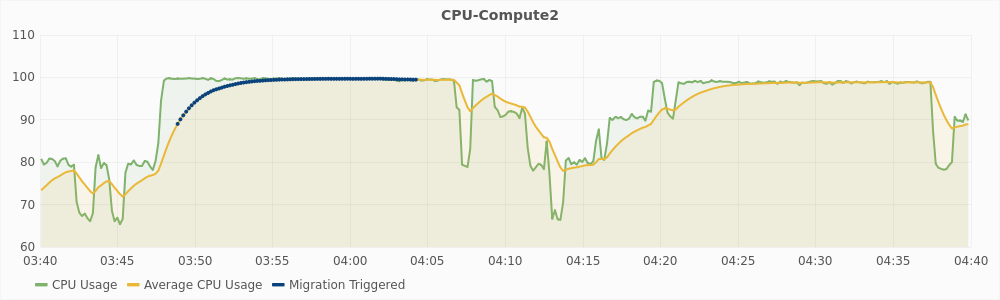
\includegraphics[width=\textwidth]{cpu-migration.png}
  \caption{CPU usage of compute2 during one hour of the experiment. Blue dots show the points at which migration was triggered. X-axis represents the time at which the value was recorded, Y-axis shows the value in \%}\label{fig:cpu-mig}
\end{sidewaysfigure}

The graph in Figure \ref{fig:cpu-mig} shows the CPU usage of compute2 for one hour during the experiment. The blue dots represent the instances at which migration was triggered. Migration was disabled for this experiment, so no machines was actually migrated out of this host. In the graph, the CPU usage is 100\% in two intervals. First interval is from around time 3:47 to 4:06 (interval1) and the second interval is from around 4:21 to 4:38 (interval2). However, migration is triggered only during interval1. This implies that there was a hotspot due to CPU utilization only during interval1 and not during interval2.

\begin{figure}[!htbp]
  \centering
  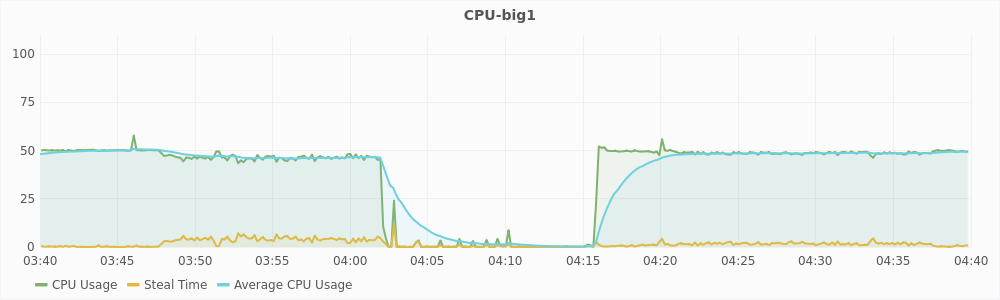
\includegraphics[width=\textwidth]{cpu-big1.png}
  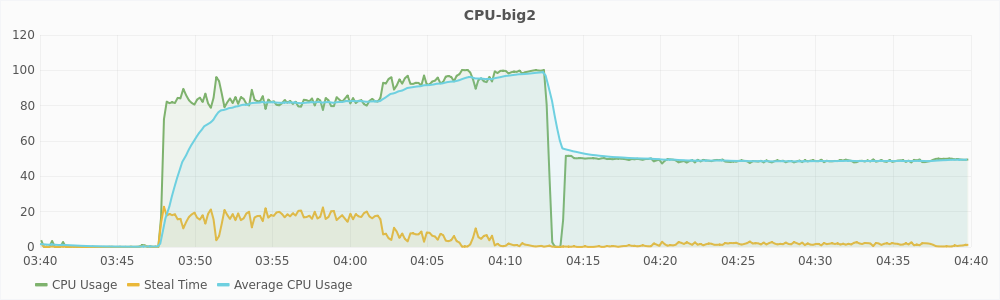
\includegraphics[width=\textwidth]{cpu-big2.png}
  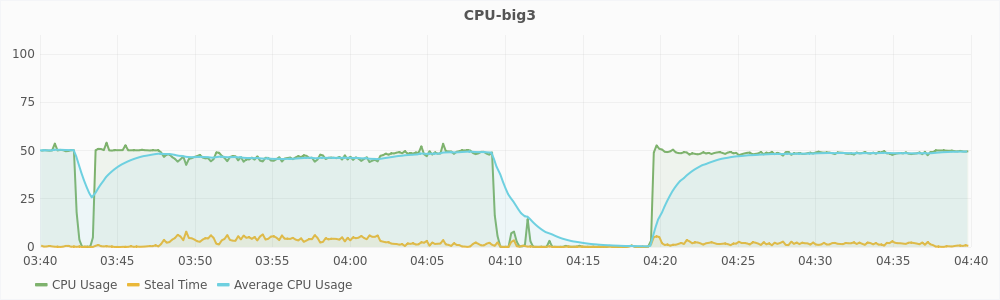
\includegraphics[width=\textwidth]{cpu-big3.png}
  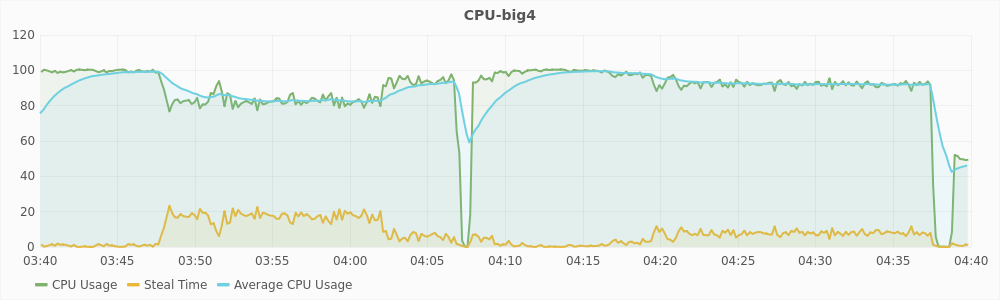
\includegraphics[width=\textwidth]{cpu-big4.png}
  \caption{CPU usage of all the large VMs on compute2 during 1 hour of the experiment. X-axis represents the time at which the value was recorded, Y-axis shows the value in \%}\label{fig:cpu-large}
\end{figure}

\begin{figure}[!htbp]
  \centering
  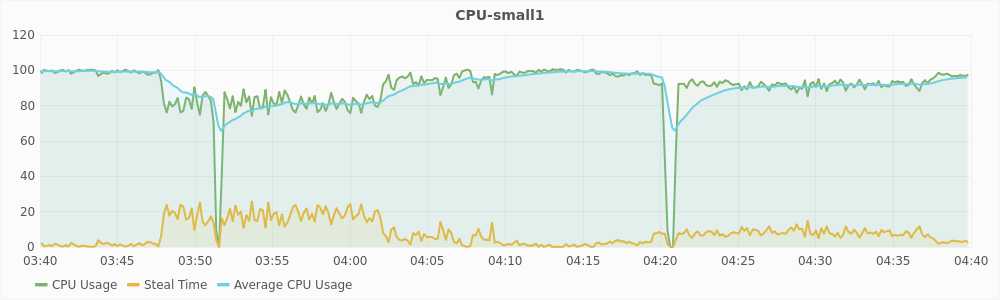
\includegraphics[width=\textwidth]{cpu-small1.png}
  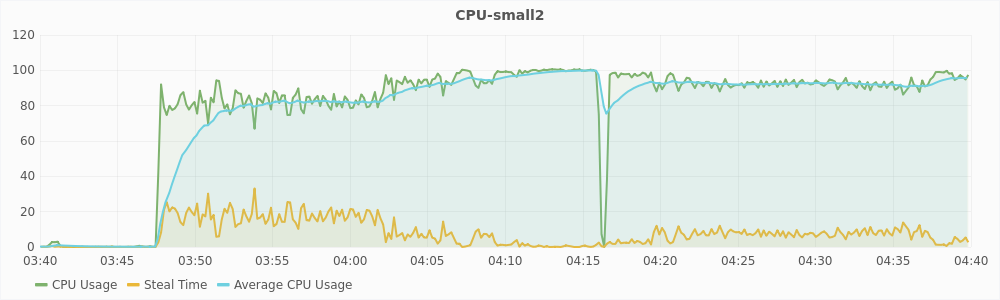
\includegraphics[width=\textwidth]{cpu-small2.png}
  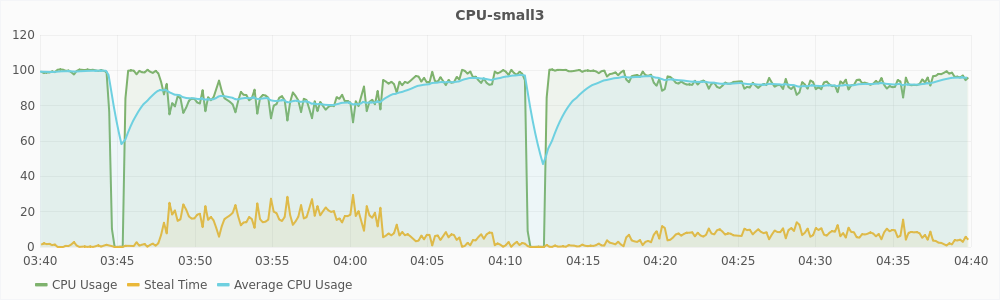
\includegraphics[width=\textwidth]{cpu-small3.png}
  \caption{CPU usage of all the small VMs on compute2 during 1 hour of the experiment. X-axis represents the time at which the value was recorded, Y-axis shows the value in \%}\label{fig:cpu-small}
\end{figure}

The graphs in Figure \ref{fig:cpu-large} and \ref{fig:cpu-small} show the CPU usage and steal time of individual virtual machines on compute2 during that one hour. For a large virtual machines, 100\% CPU usage implies that it is using two vCPUs completely and 50\% CPU usage implies that it is using only one of its two vCPUs. For a small virtual machines, 100\% CPU usage means that it is using its only vCPU completely. From the graphs, we can see that during interval1, large virtual machines are trying to use 6 vCPUs and the small virtual machines are trying to use 3 vCPUs, which is a total of 9 vCPUs. The host has only 8 physical CPUs and hence, it is overloaded. This also reflected in the steal time of the individual VMs which is higher than 10\% during interval1. During interval2, a total of 8 vCPUs are being used, which is equal to the number of the physical CPUs, and hence there is no overload. The steal time of the VMs are also low and migration is not triggered. These observations show that steal time is an appropriate metric for determining CPU hotspots.



\subsection{Analyzing the CUSUM algorithm}
Figure \ref{fig:etcd} shows a graph of one hour time duration of the experiment. The red dots in the graph mark the different points at which etcd was updated with the value of used memory for the host compute2. It is evident from the graph that the algorithm is successful in filtering sudden changes in the value of load memory and only updates etcd when the load profile has changed. In the one hour time duration, etcd was updated 13 times. Without the filtering algorithm, etcd would have been updated once in every 10 seconds i.e.\ 360 time in an hour, which is about 28 times more than the filtering algorithm. Overall during the 17 hour run of the experiment, etcd was updated just 266 times.
\begin{sidewaysfigure}[!htbp]
  \centering
  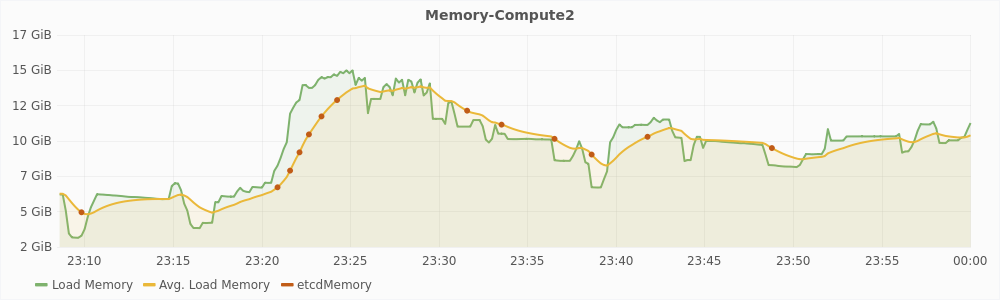
\includegraphics[width=\textwidth]{etcd-mem.png}
  \caption{Graphs showing the points at which etcd is updated. X-axis represents the time at which the value was recorded, Y-axis shows the value.}\label{fig:etcd}
\end{sidewaysfigure}

\subsection{Memory and CPU Footprint of DRS}
\begin{figure}[!htbp]
  \centering
  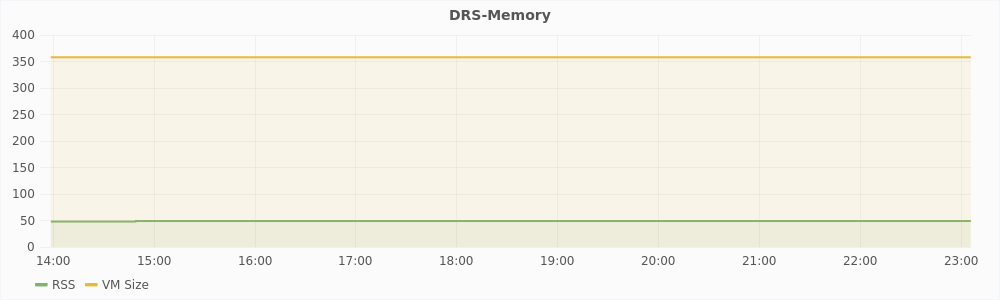
\includegraphics[width=\textwidth]{mem-self.png}
  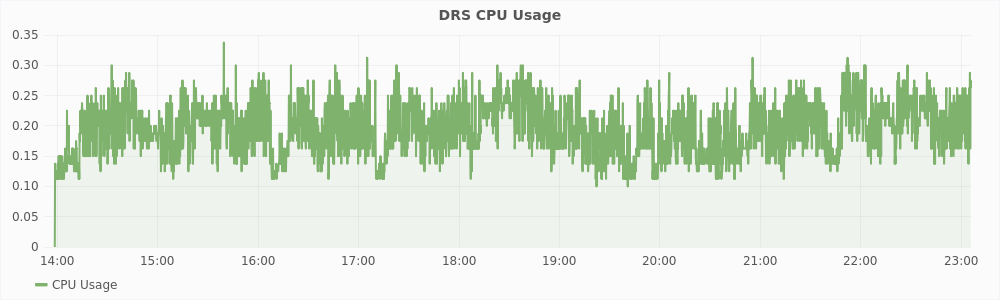
\includegraphics[width=\textwidth]{cpu-self.png}
  \caption{Graphs showing the CPU and memory used by the DRS. The memory usage is shown in MBs abd CPU usage in \%}\label{fig:self}
\end{figure}

Graphs in Figure \ref{fig:self} show the resource usage statistics of the DRS algorithm. As we can see, the CPU usage is always less then 0.35\% which is almost negligible. The memory used by the DRS algorithm is 50MB with the entire virtual memory size of the software being just 350MB.

\section*{Summary}
In this chapter, we described our experimental setup and compared the resource utilization without autoballooning with the case when autoballooning was enabled. We looked at the effectiveness of steal time in identifying CPU hotspots. We also saw the performance of the CUSUM algorithm which is used to filter sudden changes in the resource usage from affecting decision making of the DRS algorithm. We also looked at the resources consumed by our implementation of the DRS algorithm.

\chapter{Conclusions}
\label{chap:conclusions}

\section{Summary}
Resource overcommitment is an essential technique for efficient use of resources in a cloud infrastructure. There are several hurdles in overcommitment which have not been addressed completely yet. Most of the studies in this field focus on just a part of the problem, but do not solve it as a whole. The subproblems that have attracted most attention is the optimal placement of virtual machines depending on their demands. But many of these studies do not take the dynamic nature of resource demand of the VMs or the performance degradation during live migration into account. Through this thesis, we have tried to solve this problem by taking the whole picture into account, and not just a part of it.

In this thesis, we have identified some of the major problems faced in overcommitment of CPU and memory resources in a virtualized environment. We have described some of the relevant work done in this area and their limitations. We have proposed an approach and architecture to build a decentralized distributed resource scheduler to manage the cloud resources under overcommitment. The DRS is designed to be horizontally scalable and has no single point of failure. We have also implemented a complete DRS system for QEMU-KVM virtualization platform. The implementation of the autoballooning and monitoring component have been described in detail and their performance has been analyzed by experimentation.

Our implementation is open-source and the code for it can be found here:
\begin{center}
\url{https://github.com/shivanshuag/thesis-code}
\end{center}

\section{Future Work}
Although we have demonstrated that our technique for autoballooning is efficient, there are still some limitations to this approach which need to be addressed. 

\subsection{Limitation of Memory Ballooning}
The balloon driver is used to modify the amount of memory a VM has. This might have some unintended affects on the processes running inside the VM. A new process starting on the guest may require more memory than is present(because some amount of memory has been ballooned out) and crash if it does not get that memory. In some cases, if no available memory is left inside the guest, and the guest does not have swap space, the Linux OOM killer may be activated to kill some of the processes and reclaim memory. This is a rare situation and requires that either there is no swap device, or swap memory is exhausted.

Ideally, the memory ballooning process should be totally transparent to the guest VM. Doing this is a non-trivial task which might require exposing the memory allocation requests inside the guest VM to the host.

\subsection{Supporting More Resource Types}
The DRS we have built right now supports balancing of only CPU and memory resources. Other resources like the network bandwidth and disk i/o can also be overcommited and can be taken into account for balancing and migration.

\subsection{Multiple Migrations}
In our DRS, the migration service considers only single migrations to resolve hotspots. Sometimes, multiple migrations may be required to resolve a single hotspot. This will involve coordination between more than two machines for migration. Strategies to make this process effective and beneficial need to be explored.

\begin{singlespace}
\cleardoublepage
\phantomsection \label{listoffig}
\addcontentsline{toc}{chapter}{References}
\renewcommand\bibname{References}
\printbibliography
\nocite{*}
\end{singlespace}

\end{document}
